% change the aspect ratio to 169 for 16:9 aspect ratio
% otherwise remove option completely for 3:2 ratio.
\documentclass[aspectratio=169]{beamer}
\usepackage[utf8]{inputenc}
\usepackage{amsmath}
\usepackage{amsfonts}
\usepackage{graphicx}
\usepackage{braket}


\usetheme{CambridgeUS}

\useinnertheme{rectangles}

% Depending on whether you want dark or light
% theme you can change the style file, 
% drexel-light.tex for light theme and
% drexel-dark.tex for dark theme
\definecolor{drylo}{RGB}{255, 198, 0}
\definecolor{drybl}{RGB}{0,47,108}
 
\definecolor{drblk}{RGB}{0,0,0} 


\setbeamercolor{title}{fg=drybl,bg=drylo}
\setbeamercolor{subtitle}{fg=drybl,bg=drylo}
\setbeamercolor{frametitle}{fg=drybl,bg=drylo!70}
\setbeamercolor{section in head/foot}{bg=drylo}
\setbeamercolor{section in head/foot}{fg=drybl}
\setbeamercolor{subsection in head/foot}{bg=drybl}
\setbeamercolor{author in head/foot}{bg=drylo}
\setbeamercolor{author in head/foot}{fg=drybl}
\setbeamercolor{date in head/foot}{fg=white,bg=drblk}
\setbeamercolor{title in head/foot}{fg=drylo,bg=drybl}

\setbeamercolor{local structure}{fg=drylo,bg=drybl}


\author{Sean C. Lewis}
\title{Effects of Early Forming Massive Stars}

\date{\today} 
\subject{Physics} 

% depending on dark or light theme use _black or _white pdf for drexel logo.
% These logos are obtained from https://drexel.edu/identity/drexel/logotypes/


% Two graphics side by side
%\titlegraphic{%
%    \hfill
%   
\includegraphics[height=0.7cm]{../images/Drexel_horizontal_black.pdf}%
%    \hfill%
%    
\includegraphics[height=1cm]{../images/EXO_logo.pdf}%
%}

%%%%% Only Drexel
\titlegraphic{%
    %\hfill
    
\includegraphics[height=0.7cm]{../images/Drexel_horizontal_black.pdf}%
    %
\includegraphics[height=0.7cm]{../images/Drexel_horizontal_white.pdf}%
}


\begin{document}

\titlepage

\section{Hypothesis}
\begin{frame}{Early Forming Massive Stars}{Disruption of gas collapse, star formation, and cluster assembly}
    \begin{itemize}
        \only<1,2,3,4>{\item The feedback from massive stars likely dominates the self-regulation of star formation.}
        \only<2,3,4>{\item Gas evacuation (via stellar feedback) is crucial to the completion of star cluster assembly.\footnote{Bressert et al. 2010; Longmore  et al. 2014; Grudi\'c et al. 2018; Dobbs et al. 2022}}
        \only<3,4>{\item \emph{How} gas is removed (rapidly, or slowly) may affect cluster structure.\footnote{Smith et al. 2013; Portegies Zwart et al. 2010; Banjeree \& Kroupa 2017}}
        \only<3,4>{\item []}
        \only<4>{\item What about \emph{when} massive stars form? Using our computational model we test the effects of early forming massive stars.}
    \end{itemize}
\end{frame}

\section{Torch}
%
\begin{frame}{Torch}{Stars from gas}
    \begin{itemize}
        \item Couples N-body, stellar evolution, and feedback in \texttt{AMUSE} \\ with self-gravitating magnetized gas in MHD code \texttt{FLASH}.
        \item []
        \item Resolved dynamics of stars and gas; study star cluster formation within collapsing GMCs.
        \item []
        \item Form stars from sink particles which each have a randomized star mass list sampled from the Kroupa IMF.$^[$\footnote{Kroupa 2001}$^]$
    \end{itemize}
\end{frame}



\section{Experiment}
\begin{frame}{A Controlled Experiment}{}
    \begin{columns}
        \begin{column}{0.45\textwidth}
            \begin{figure}[h!]
                \centering
                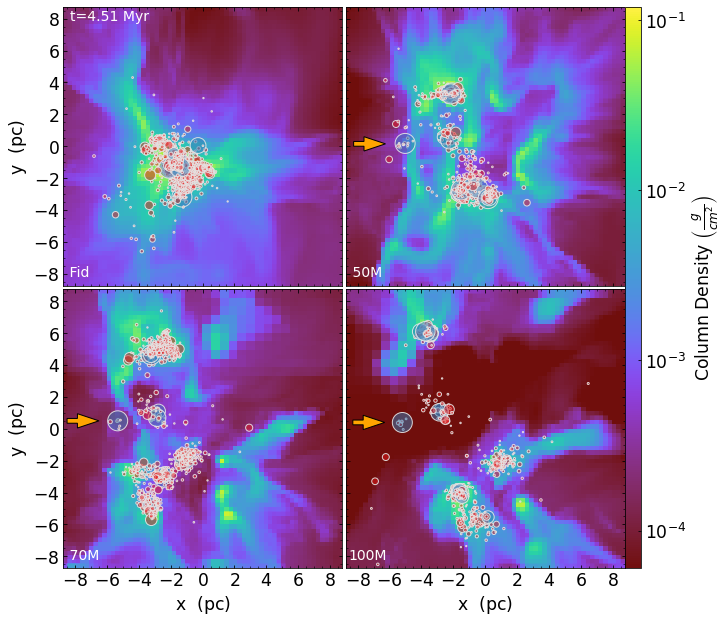
\includegraphics[width=\linewidth]{../images/density_grid.png} \\
                Lewis et al. 2023
                \label{fig:density}
            \end{figure}
        \end{column}
        \begin{column}{0.35\textwidth}
            
            \begin{figure}[h!]
                \centering
                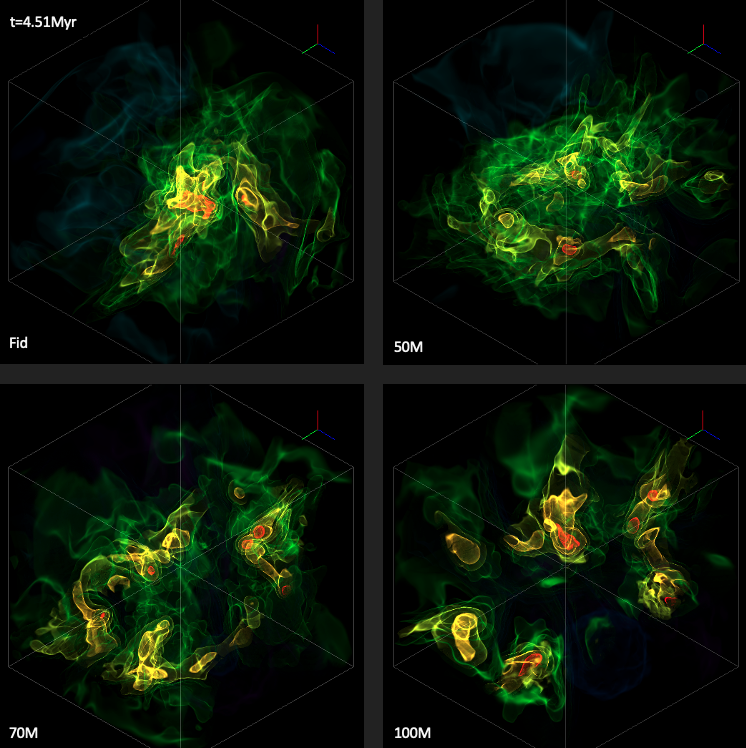
\includegraphics[width=\linewidth]{../images/paper1-snapshot-volume-render.png} \\
		
                \label{fig:volume}
            \end{figure}
        \end{column}
    \end{columns}
\end{frame} 

\section{Results}

\begin{frame}{Effects on Gas Energy}{}
    \begin{columns}
        \begin{column}{0.45\textwidth}
            \begin{figure}[h!]
                \centering
                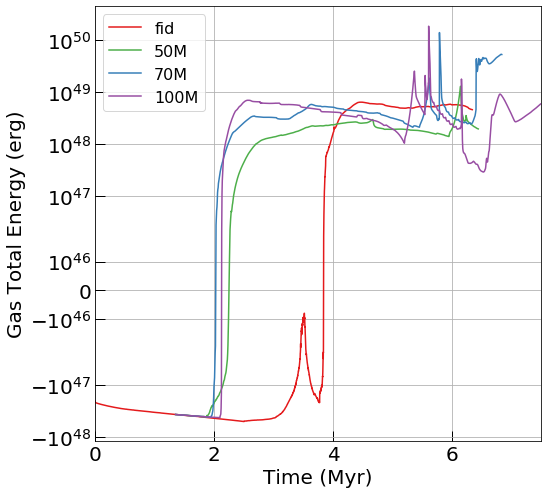
\includegraphics[width=\linewidth]{../images/global_gas_total_energy_fixes.png} \\
                \label{fig:energy}
            \end{figure}
        \end{column}
        \begin{column}{0.45\textwidth}
            \begin{figure}[h!]
                \centering
                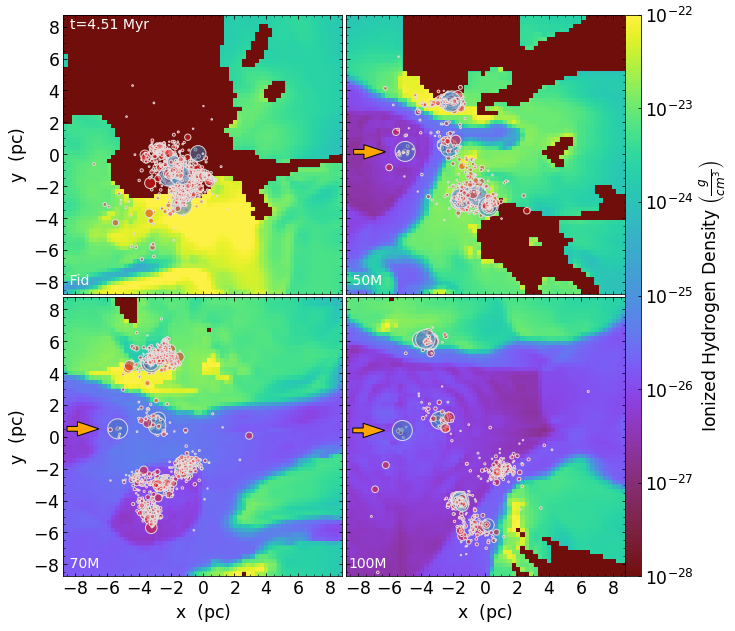
\includegraphics[width=\linewidth]{../images/ionized_H_slice.png} \\
                \label{fig:ionized}
            \end{figure}
        \end{column}
    \end{columns}
\end{frame} 


\begin{frame}{Effects on Gas Accretion and Star Formation}{}
    \begin{columns}
        \begin{column}{0.45\textwidth}
            \begin{figure}[h!]
                Gas Satisfying Jeans Criterion
                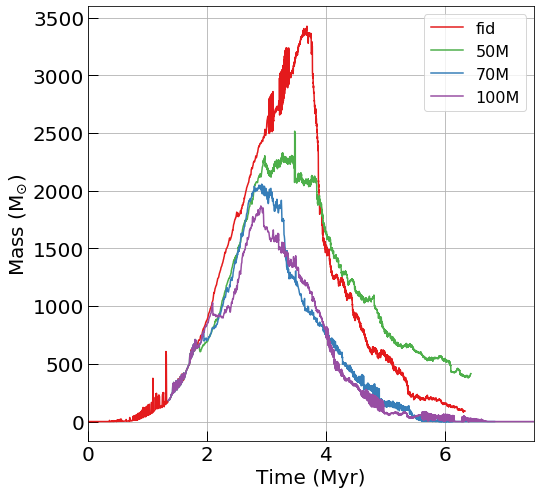
\includegraphics[width=\linewidth]{../images/jeans_gas_mass.png} \\
                \label{fig:jeans_mass}
            \end{figure}
        \end{column}
        \begin{column}{0.45\textwidth}
            \begin{figure}[h!]
            	Cumulative Stellar Mass
                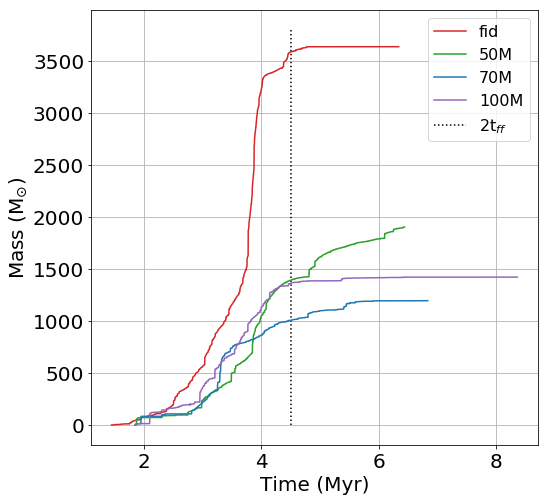
\includegraphics[width=\linewidth]{../images/cumulative_stellar_mass_fixes.png} \\
                \label{fig:cum_mass}
            \end{figure}
        \end{column}
    \end{columns}
\end{frame} 

\begin{frame}{Effects on Gas Accretion and Star Formation}{}
    \begin{columns}
        \begin{column}{0.42\textwidth}
            \begin{figure}[h!]
                \centering
                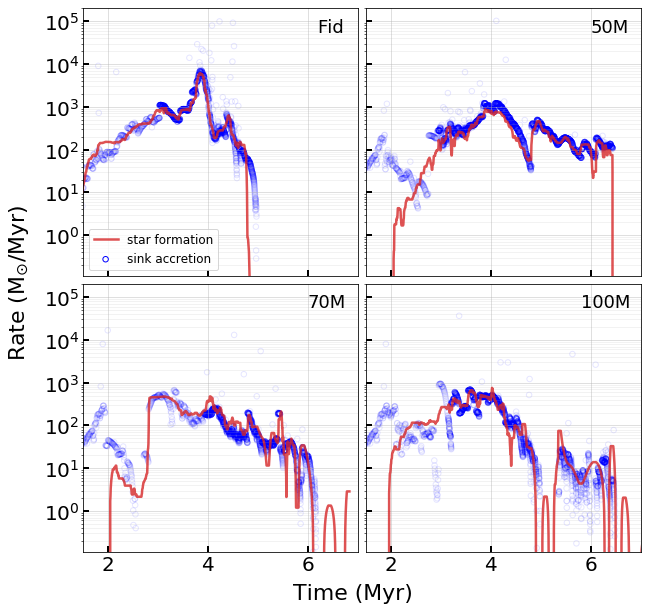
\includegraphics[width=\linewidth]{../images/sink_accretion_star_formation_rates.png} \\
                \label{fig:sink_star_rates}
            \end{figure}
        \end{column}
        \begin{column}{0.42\textwidth}
            Early forming massive stars reduces sink accretion and star formation rates.
            \only<1>{\vspace{3.2cm}}
            \only<2>{
            \begin{table}[!htb]
                \begin{tabular}{cc}
                    \hline
                    Run & $\braket{\epsilon_{ff}}$ \\
                    \hline
                    Fid & 0.23 \\
                    50M & 0.08 \\
                    70M & 0.03 \\
                    100M & 0.04 \\
                    \hline
                \end{tabular}
            \end{table}
            }
        \end{column}
    \end{columns}
\end{frame} 



\begin{frame}{Effects on Star Clustering, Cluster Assembly}{}
    \begin{columns}
        \begin{column}{0.45\textwidth}
            \begin{figure}[h!]
                \centering
                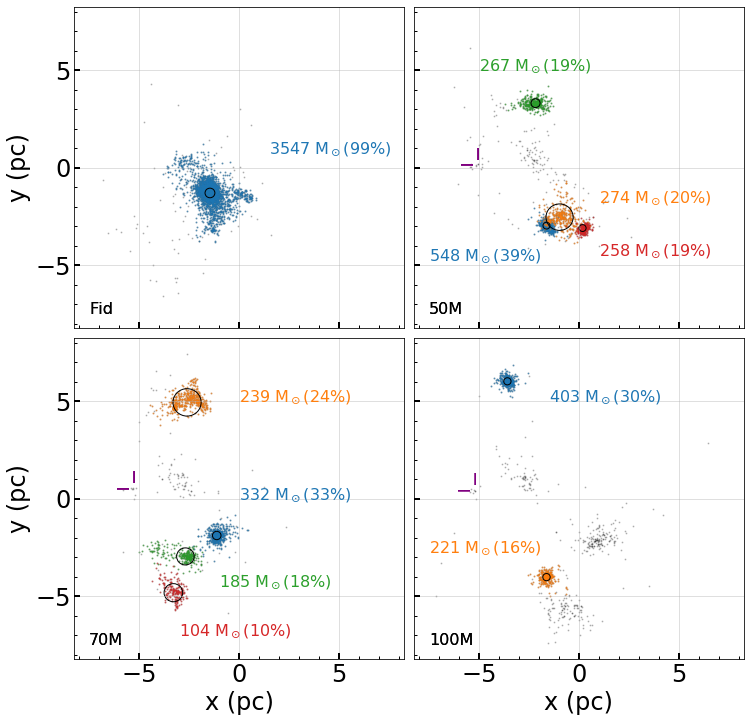
\includegraphics[width=\linewidth]{../images/cluster_grid.png} \\
                \label{fig:cluster_grid}
            \end{figure}
        \end{column}
        \begin{column}{0.45\textwidth}
            \begin{itemize}
              \item DBSCAN to identify cluster with at least 50\% bound members and 100~M$_\odot$ at 2$\tau_{\rm ff}$.
              \item Clusters in runs with early massive stars are less massive and more fragmented compared to the fiducial run.  
            \end{itemize}
	    \begin{table}[!htb]
            	\tiny
 		%\centering
 		%\caption{Cluster statistics at $2\tau_{\rm ff}$.}
 		\label{tab:cluster_stats_2tff}
 		\begin{tabular}{lcccc} 
  			\hline
  			Run & Mass in Clusters & Frac Mass & r$_{\rm h}$ MMC & E$_{\rm bind}$ MMC \\
  			& 10$^3$ $M_{\odot}$ & $M_{c}/M_{tot}$ & pc & $10^{46}$ erg\\
  			\hline
  			Fid & 3.6 & 0.99 & 0.25 & -140 \\
  			50M & 1.4 & 0.97 & 0.17 & -12 \\
  			70M & 0.86 & 0.85 & 0.21 & -4.2 \\
  			100M & 0.62 & 0.46 & 0.18 & -3.8 \\
  			\hline
 		\end{tabular}
	    \end{table}
        \end{column}
    \end{columns}
\end{frame} 



\begin{frame}{Effects of Early Forming Massive Stars}{}
    \begin{itemize}
        \item Significantly disrupt the natal gas structure, resulting in premature unbinding of GMC.
        \item []
        \item The star formation rate per free-fall time is suppressed by up to a factor of seven, reducing the total mass of stars formed.
        \item []
        \item Stifle the hierarchical assembly process of massive star clusters, instead promoting the formation of spatially separate and more loosely bound subclusters.
        % Like ignoring the galactic environment, starting from spherical or cylindrical conditions.
    \end{itemize}
\end{frame}
%
%
%
%
% 
\begin{frame}{The Problem with Initial Conditions}{}
    \begin{itemize}
        \item Self consistent galactic scale simulations with resolution down to sub-tenth parsec scales and include Nbody individual stellar dynamics and individual stellar feedback all at once? A little tough.
        \item []
        \item Creating our own isolated clouds from scratch? ``Creative liberties..."
        % Like ignoring the galactic environment, starting from spherical or cylindrical conditions.
    \end{itemize}
\end{frame}
%
%
%
\section{Motivation}
%
%
%
%
%\begin{frame}{Stars From ``Realistic" Clouds}{}
%    \begin{itemize}
%        \item Clouds that formed under the influence of galactic dynamics.
%        \item []
%        \item Track dynamics and feedback of individual stars.
%        \item []
%        \item High resolution to quantify star-gas interactions.
        % With Torch, we can already do the last two points.
        % So what we really need are some clouds from galactic simulations
%    \end{itemize}
%\end{frame}
%
%
%
\section{VorAMR}
%
%
% 
\begin{frame}{Clouds from Galactic Simulations}
	\begin{figure}[h!]
                \centering
                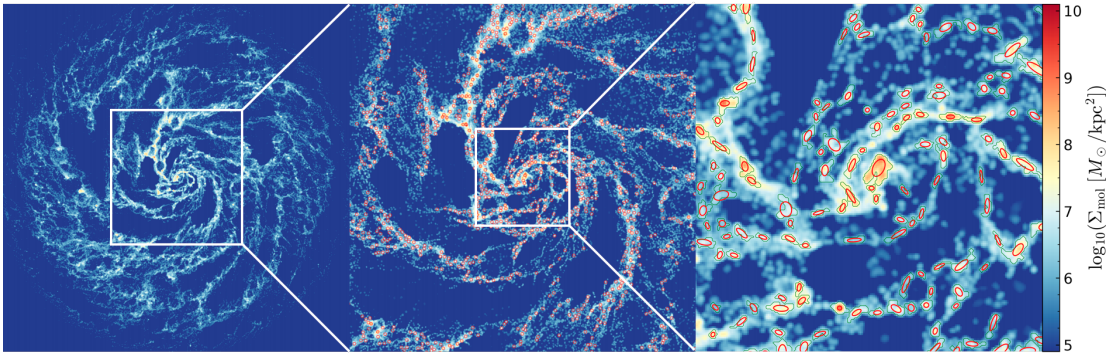
\includegraphics[width=\linewidth]{../images/AREPO_galaxy.png} \\
                GMC identification\footnote{Li, H. et al. 2020}
                \label{fig:arepo_galaxy}
	\end{figure}
	% Also have Cloud-Factory Rowen Smith (2019)
\end{frame}
%
%
%
%
%
\begin{frame}{From AREPO to FLASH} {Try CIC Mapping?}
    \begin{columns}
        \begin{column}{0.35\textwidth}
            \begin{figure}[h!]
                \centering
                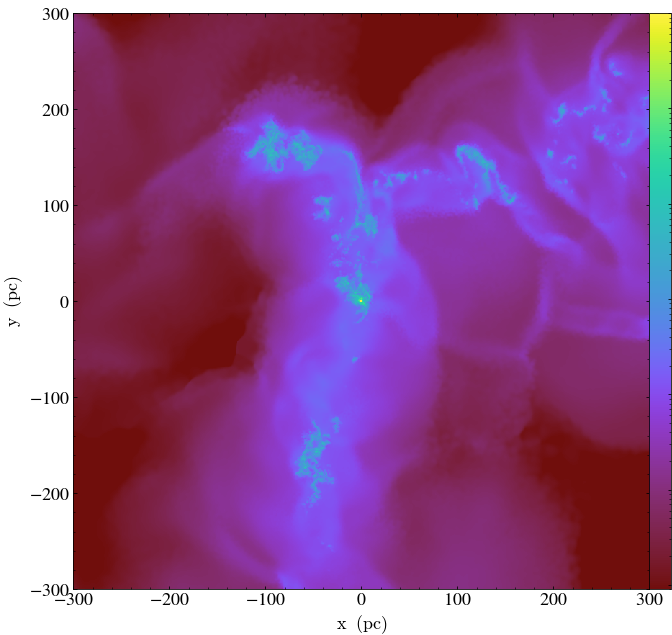
\includegraphics[width=\linewidth]{../images/AREPO_cloud.png} \\
                Cloud from raw AREPO data \\
                represented using SPH kernels
                \label{fig:voronoi_example}
            \end{figure}
        \end{column}
        \begin{column}{0.35\textwidth}
            %
            \begin{figure}[h!]
                \centering
                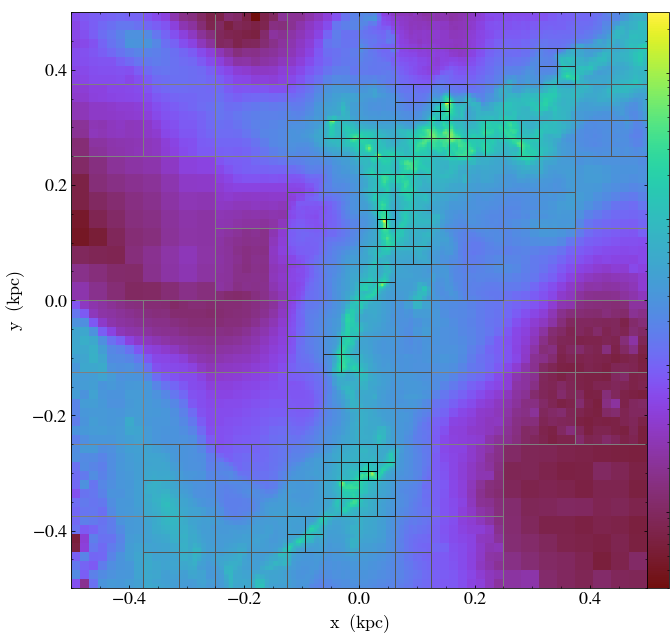
\includegraphics[width=\linewidth]{../images/cloud_in_cell_projection_lvl8.png} \\
                Cloud-in-cell mapping onto AMR FLASH grid
                \label{fig:amr_example}
            \end{figure}
        \end{column}
    \end{columns}
\end{frame} 
%
%
%
%
%
\begin{frame}
    \centering
    \only<1>{\begin{figure}[h!]
        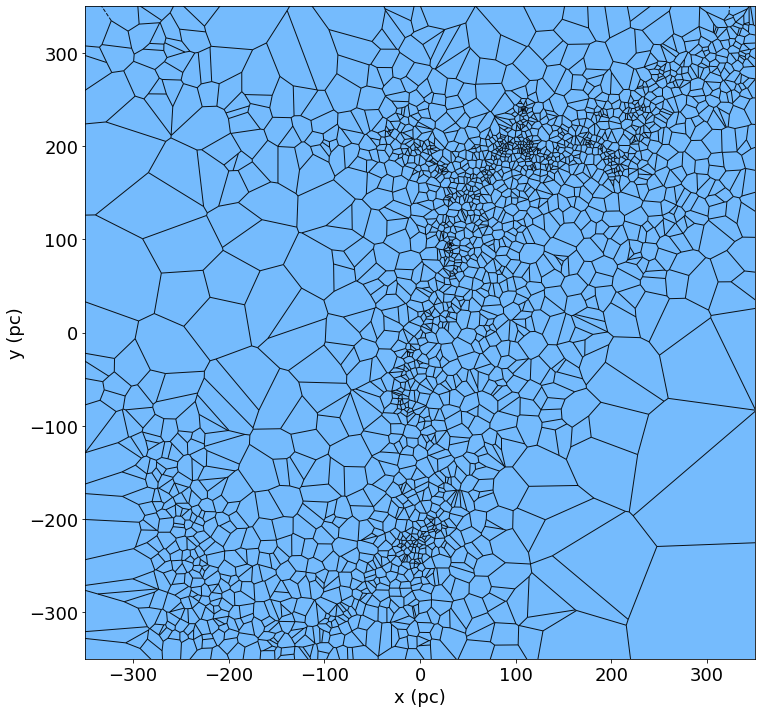
\includegraphics[width=0.5\linewidth]{../images/voronoi_mesh.png}
    \end{figure}}
    \only<2>{\begin{figure}[h!]
        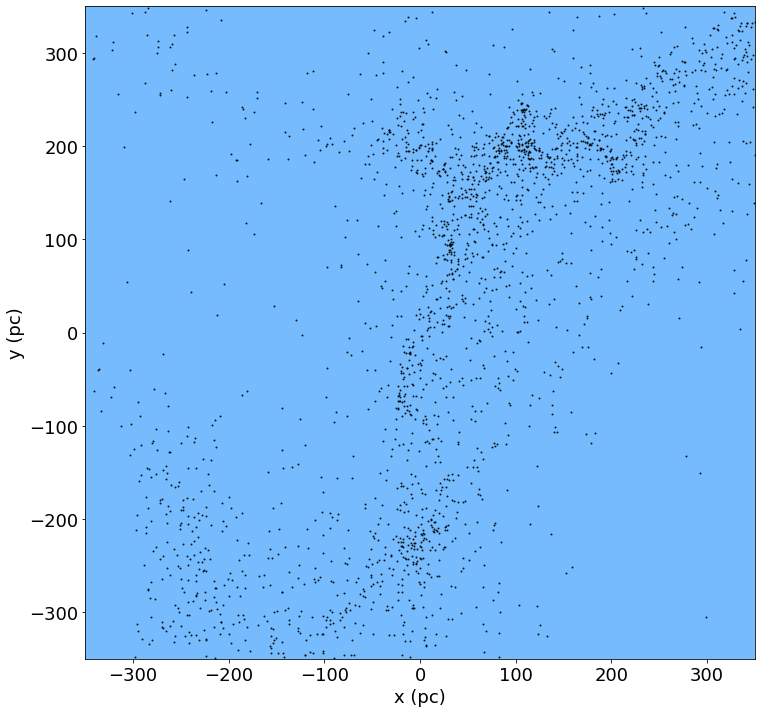
\includegraphics[width=0.5\linewidth]{../images/voronoi_centers.png}
    \end{figure}}
    \only<3>{\begin{figure}[h!]
        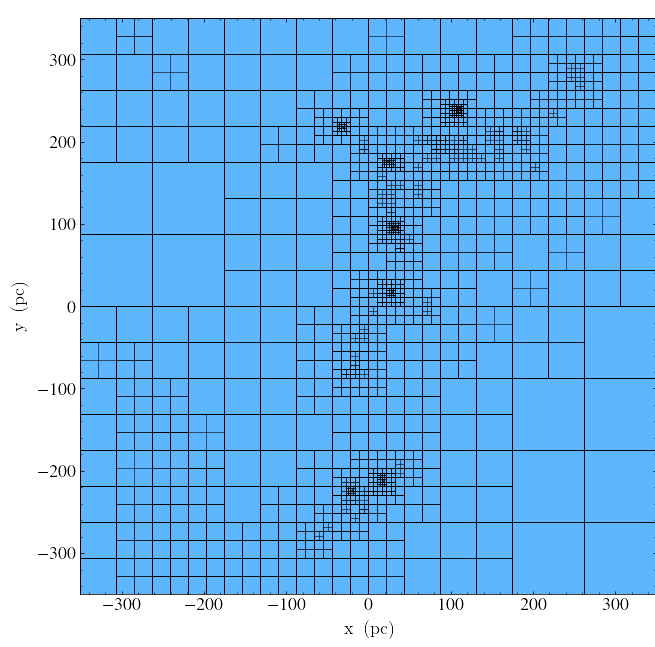
\includegraphics[width=0.5\linewidth]{../images/amr_grid_from_voronoi.png}
    \end{figure}}
    \only<4>{\begin{figure}[h!]
        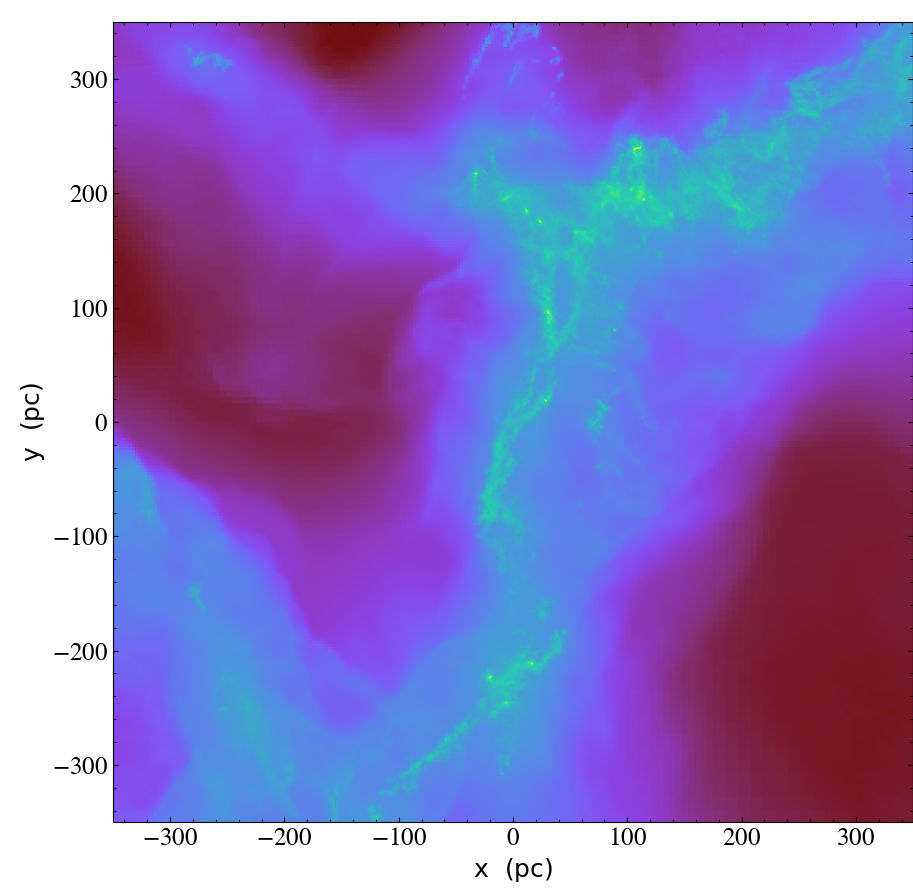
\includegraphics[width=0.5\linewidth]{../images/VorAMR_hdf5_chk_0001_Projection_z_dens.png}
    \end{figure}}
\end{frame}

\begin{frame}{Voronoi Mesh to AMR Grid} %{Subtitle not required in this slide}
    \begin{columns}
        \begin{column}{0.45\textwidth}
            \begin{figure}[h!]
                \centering
                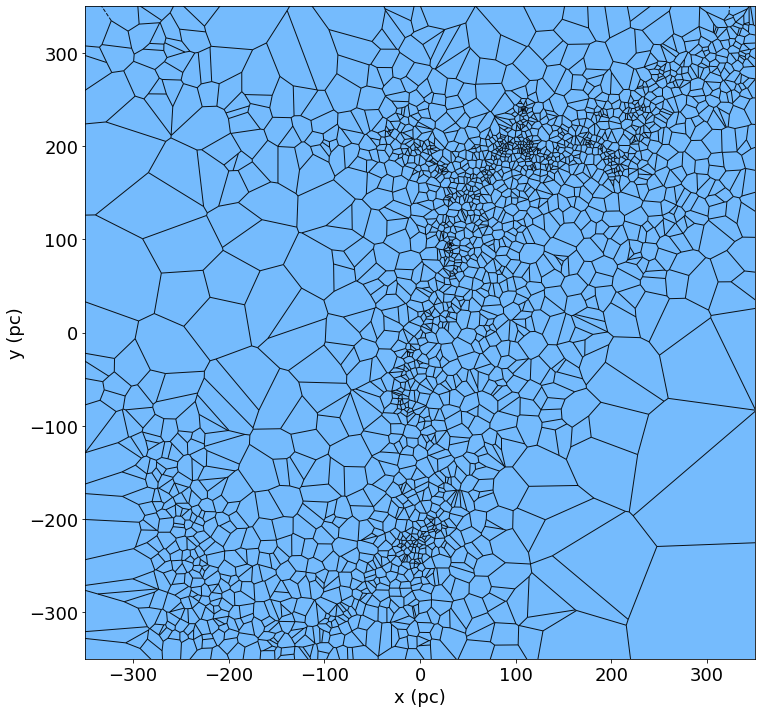
\includegraphics[width=\linewidth]{../images/voronoi_mesh.png}
                %\caption{Voronoi mesh from 20 points}
                \label{fig:voronoi_example}
            \end{figure}
        \end{column}
        \begin{column}{0.44\textwidth}
            %
            \begin{figure}[h!]
                \centering
                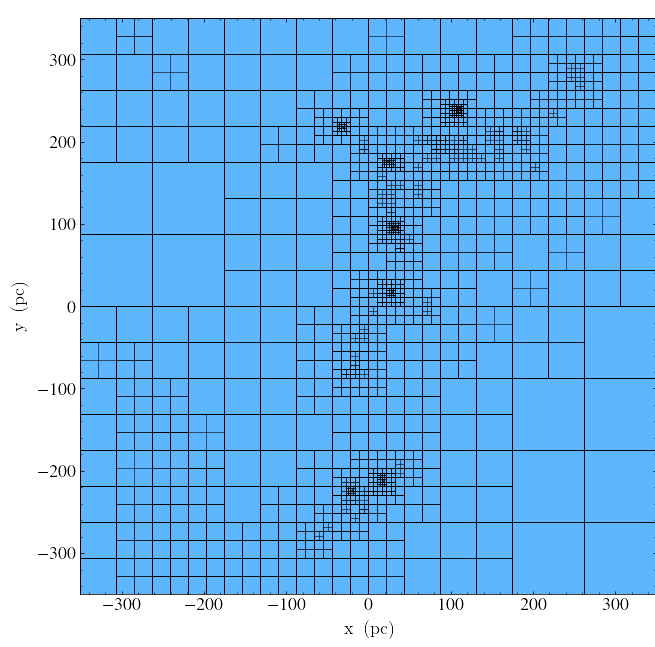
\includegraphics[width=\linewidth]{../images/amr_grid_from_voronoi.png}
                %\caption{AMR grid from 20 points}
                \label{fig:amr_example}
            \end{figure}
        \end{column}
    \end{columns}
\end{frame} 
%
%
%
%
%
%\begin{frame}{Clouds in Reality and... Not}{}
%    \begin{columns}
%        \begin{column}{0.35\textwidth}
%            \begin{figure}[h!]
%                \centering
%                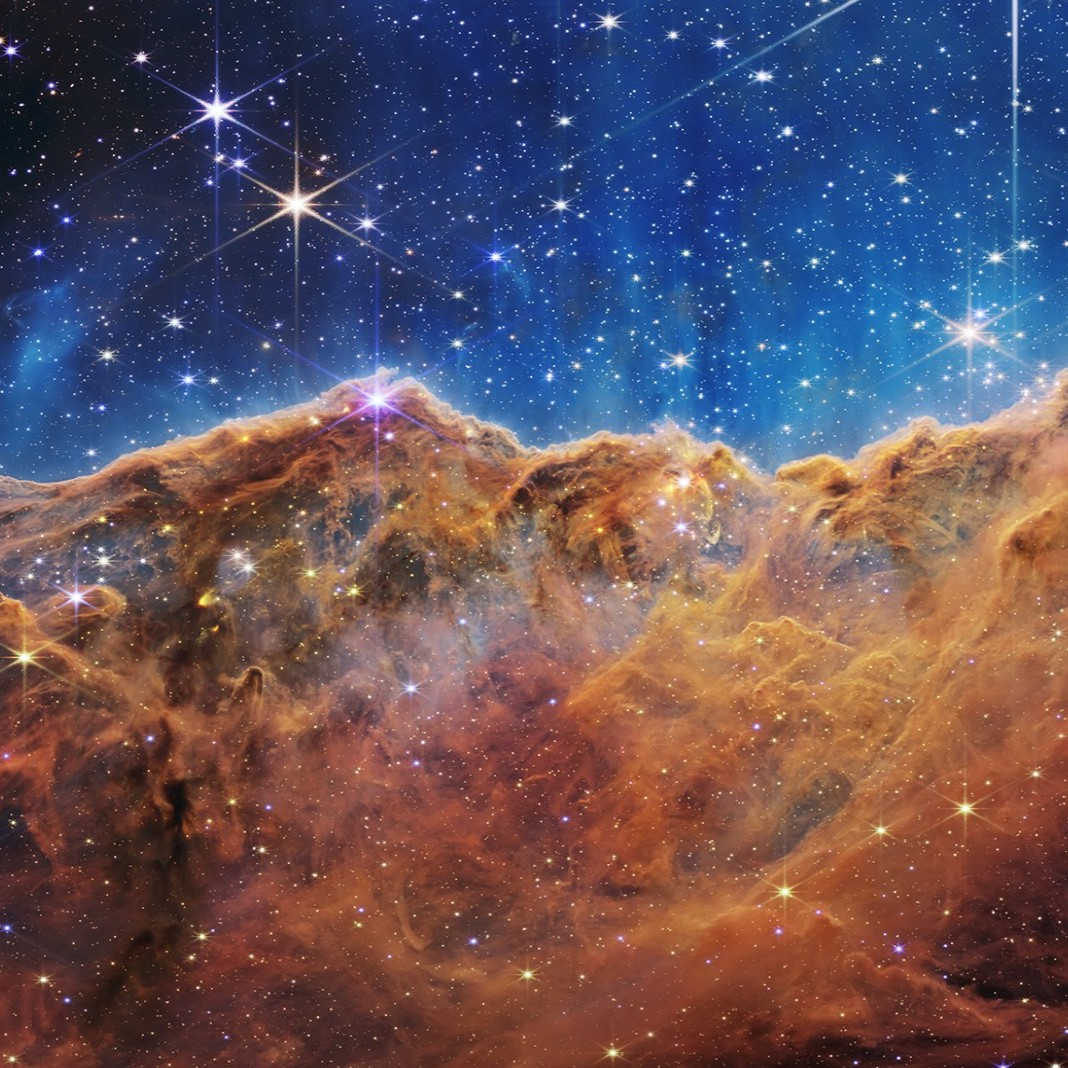
\includegraphics[width=\linewidth]{../images/jwst.jpg} \\
%                NASA; Carina Nebula
%                \label{fig:jwst}
%            \end{figure}
%        \end{column}
%        \begin{column}{0.35\textwidth}
%            %
%            \begin{figure}[h!]
%                \centering
%                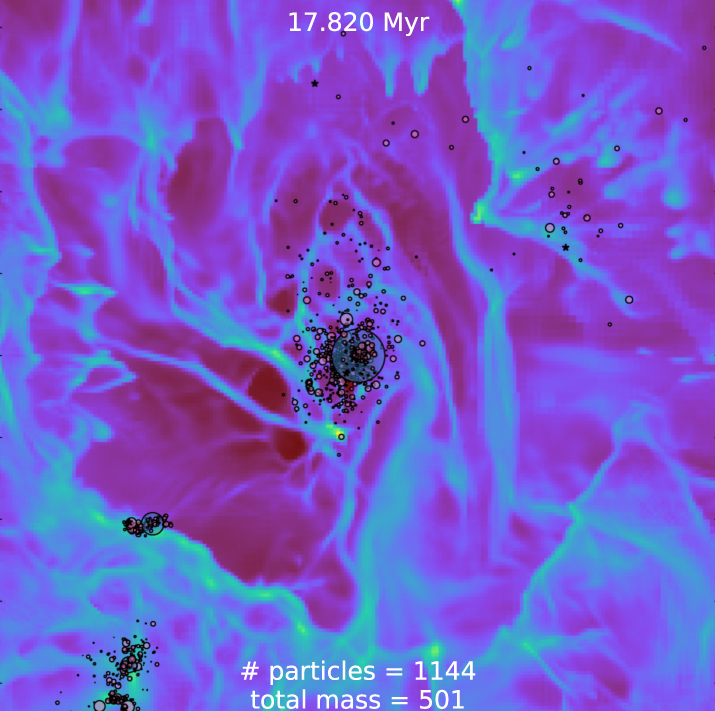
\includegraphics[width=\linewidth]{../images/josh_torch_run.jpeg} \\
%                Wall et al. 2020
%                \label{fig:torch}
%            \end{figure}
%        \end{column}
%    \end{columns}
%\end{frame} 
%
%
%
%
%
\begin{frame}{VorAMR: Logic path}
	\begin{figure}[h!]
                \centering
                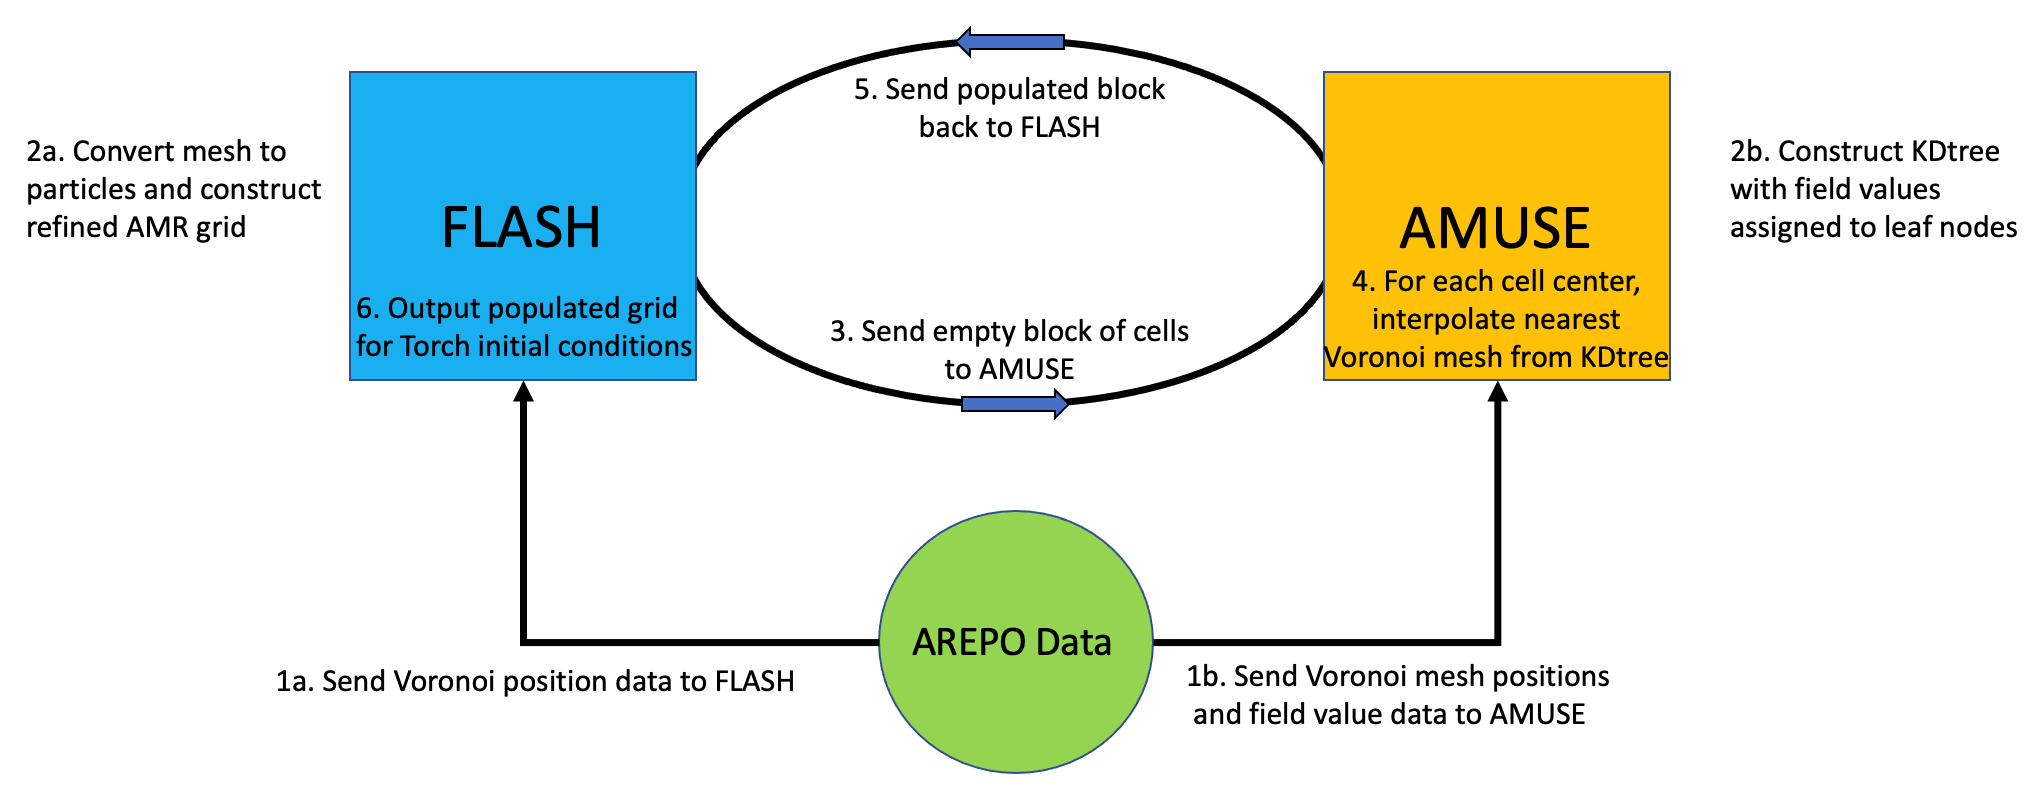
\includegraphics[width=\linewidth]{../images/voramr_logic.png} \\
                \label{fig:voramr_logic}
	\end{figure}
\end{frame}
%
%
%
%
%
% Conversion from Voronoi to AMR grid also allows for better visualizations in yt (which approximates voronoi mesh as sph kernels)
\begin{frame}{VorAMR: The Big Wins}{}
    \begin{itemize}
    	\item Significantly expands Torch's horizon and moves Torch to "completion".
	\item []
    	\item Opens wide avenue of collaboration; code bases do not have to be exclusive! 
	\item []
	\item More accurate visualizations (no more estimating Voronoi meshes as SPH kernels in \texttt{yt}).
        % With Torch, we can already do the last two points.
        % So what we really need are some clouds from galactic simulations
    \end{itemize}
\end{frame}
%
%
%
%
%
\begin{frame}{}
	\centering Thank You! \\ - \\ Questions?
\end{frame}

\begin{frame}{Appendix}
	\begin{equation}\label{eqn:sfe}
		\epsilon_{\text{ff}} = \dot{M}_{*}\frac{t_{\text{ff}}}{M_{\text{g}}}
	\end{equation}
\end{frame}

\end{document}

